\documentclass[00-livre-main.tex]{subfiles}
\begin{document}

\chapter{The Equation of a Line in the Plane}


Let's recall the idea of \emph{the plane} from classical geometry: the plane is like a flat sheet of drawing paper, which extends indefinitely in all directions without bound.
It is the playground for lots of serious considerations from high school: points, lines, circles, triangles, rectangles, and various other doodles live in it.
I say \emph{in} it rather than \emph{on} it, because all of those objects really have their existence inside the plane.
If we were to say ``on the plane'' then one might think of them as sitting on top of the paper, where a light breeze might move them about.
No, those things live inside the plane just as sure as you and I live inside the universe.

And while all of that is evocative and romantic, it doesn't make doing mathematics any easier.
Our aim in this first chapter is to do some concrete mathematics: we want to figure out how to describe a single line in the plane very carefully.
To do this, we will use tools that Ren\'{e} Descartes taught us: coordinates.
Better yet, we will use an update of the idea and introduce \emph{vectors}.
Our work has to rely on something, so at some points we will make use of geometry facts you learned in high school.
But for all of the points and vectors, angles and dot products, we will go straight to the heart of a single important question:

\begin{quotation}
\textbf{\large How can we clearly describe a single line in the plane with an equation?}
\end{quotation}

\clearpage

\section*{Points, Vectors, and Vectors}


You have likely seen the idea of \emph{Cartesian coordinates} on the plane before. To be clear, let's set things down carefully. In the plane, we choose a pair of perpendicular lines which meet at a point $O$. This special point is called the \emph{origin}. Then, we choose a point $X$ on one of the lines and draw the circle centered at $O$ which passes through $X$. Note that this circle meets our two lines in two points each, four points total, one of which is the point $X$. Then, from $X$, we rotate around the circle by a quarter turn counterclockwise until we hit one of the points on the other line. This new point we will call $Y$. Are you drawing with me? Here is my picture so far.

\begin{figure}[h!]
\centering
\begin{tikzpicture}[scale=2]
\draw (-1,4/3) -- (1,-4/3);
\draw (-3/2,-9/8) -- (3/2,9/8);
\draw (0,0) circle [radius=3/4];
\draw[->] (-50:1) arc (-50:35:1);
\node [right] at (1.1,0) {rotate counterclockwise};
\node [left] at (0,0) {$O$};
\node [below] at (9/20,-13/20) {$X$};
\node [above] at (3/5,9/20) {$Y$};
\end{tikzpicture}
\end{figure}

We call the line $OX$ the \emph{$x$-axis} and the line containing $Y$ the \emph{$y$-axis}. Here comes the amazing part: we declare the circle we used to be of \emph{unit size}, and make the lines $OX$ and $OY$ into number lines! The important part is that the point $O$ should represent $0$ on both number lines, and the points $X$ and $Y$ should each represent $1$ on their lines. So, instead of marking things with $O$, $X$, and $Y$, we put down marks where $X$ and $Y$ are and label them with $1$'s, and add little arrows marked with $x$ and $y$ near the positive ``ends'' of the lines $OX$ and $OY$, respectively.

\begin{figure}[h!]
\centering
\begin{tikzpicture}[scale=1.2]
\draw[->] (-1,4/3) -- (1,-4/3);
\draw[->] (-3/2,-9/8) -- (3/2,9/8);
\draw[fill] (9/20,-3/5) circle [radius=0.03];
\draw[fill] (3/5,9/20) circle [radius=0.03];
\node [below] at (9/20,-3/5) {$1$};
\node [above] at (3/5,9/20) {$1$};
\node [right] at (1,-4/3) {\small $x$};
\node [left] at (3/2,9/8) {\small $y$};
\end{tikzpicture}
\end{figure}

Note that above I have done something a bit silly and let the picture just fall on the paper in an unusual way.
I really mean unusual as ``not usual.''
The usual way arranges the lines on the paper to match our expected horizontal ($x$) and vertical ($y$) directions.
This isn't actually required, but it is what everyone always does.
The typical picture looks like Figure \ref{fig:cartesian-coords}.


\begin{figure}[h]
\centering
\begin{tikzpicture}[scale=1.2]
\draw[->] (-2,0) -- (2,0) node[below] {\small $x$};
\draw[->] (0,-2) -- (0,2) node[left] {\small $y$};
\draw[fill] (1,0) circle [radius=0.03] node[below] {$1$};
\draw[fill] (0,1) circle [radius=0.03] node[left] {$1$};
\end{tikzpicture}
\caption{The Standard Cartesian Coordinate System}
\label{fig:cartesian-coords}
\end{figure}


Now suppose we have some point in the plane, let's call it $P$.
We can describe the location of $P$ relative to our two lines in a simple way. First, we draw a line through $P$ which is parallel to the $y$-axis and perpendicular to the $x$-axis.
The foot of this perpendicular hits the $x$-axis at some point $A$.
But this point $A$ is part of the number line $OX$, so it has an associated real number, which we will call $a$.
So the point $A$ is instead marked with the label $a$ from this number line.

Similarly, we draw a line through $P$ parallel to the $x$-axis and perpendicular to the $y$-axis.
The foot of this perpendicular hits the $y$-axis at some point $B$, which is part of the number line $OY$.
We denote the number associated to $B$ by $b$.
Again, the point is labeled with the number $b$ from the number line.

\begin{figure}[h!]
\centering
\begin{tikzpicture}[scale=1.2]
\draw[->] (-2,0) -- (2,0) node[below] {\small $x$};
\draw[->] (0,-2) -- (0,2) node[left] {\small $y$};
\draw[fill] (-1/2,3/4) circle [radius=0.03] node[below left] {$P$};
\draw[dotted] (-1/2,-2) -- (-1/2,2);
\draw[dotted] (-2,3/4) -- (2,3/4);
\draw (-.05,3/4) -- (.05,3/4) node[above right] {$b$};
\draw (-1/2,.05) -- (-1/2,-.05) node[below left] {$a$};
\end{tikzpicture}
\caption{A point $P$ and its coordinates $(a,b)$.}
\label{fig:point-coords}
\end{figure}

So, to identify the point $P$, we can instead give the pair of numbers $a$ and $b$.
These numbers are called the \emph{coordinates} of $P$.
Of course, the order of the coordinates matters, so we make what we call an \emph{ordered pair} $(a,b)$ to keep things straight, where the $x$-coordinate comes first, and the $y$-coordinate comes second. Note that in Figure \ref{fig:point-coords} the $x$-coordinate $a$ is negative, but the $y$-coordinate $b$ is postive.

This whole process is reversible, too. If we pick a pair of numbers $c$ and $d$, in order, then we can find a point in the plane which corresponds, and we can do it unambiguously. Find the spot labeled $c$ on the $x$-axis number line and construct a line perpendicular to the $x$-axis through this point. Similarly, find the spot labeled $d$ on the $y$-axis and construct a line perpendicular to the $y$-axis through this point. The two lines you just drew will meet in exactly one point $Q$, and $Q$ will have coordinates $(c,d)$.

This setup of coordinates on the plane allows us to formalize a wonderful and useful idea from physics, too.
Physicists use the concept of a \emph{vector} to describe something (like the wind) which has both magnitude or size (like how fast the air is moving)  and direction (which way the air is going).
Usually, vectors are drawn as little arrows: the arrow has a direction, and it has a length which represents its magnitude.
It is possible to draw vectors which have the same direction but different lengths, and vice versa.

We can use coordinates to describe vectors in the plane, too.
Here's how: A physicist's vector $v$ is some arrow in the plane.
That arrow has an initial point $P$, called its \emph{tail}, and a final point $Q$, called its \emph{head}.
We can write the coordinates of these points as $P = (a,b)$ and $Q = (c,d)$.

\begin{figure}[h]
\centering
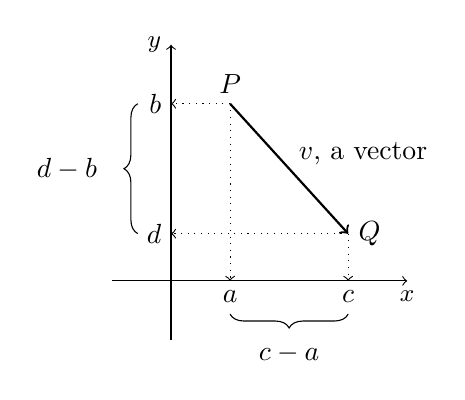
\begin{tikzpicture}[scale=1.5]
\draw[->] (-.5,0) -- (2,0) node[below] {\small $x$};
\draw[->] (0,-.5) -- (0,2) node[left] {\small $y$};
\draw[->,thick] (1/2,3/2) node[above] {$P$} -- (3/2,2/5) node[right] {$Q$};
\node [above right] at (1,18/20) {$v$, a vector};
\draw[dotted,->] (1/2,3/2) -- (1/2,0) node[below] {$a$};
\draw[dotted,->] (1/2,3/2) -- (0,3/2) node[left] {$b$};
\draw[dotted,->] (3/2,2/5) -- (3/2,0) node[below] {$c$};
\draw[dotted,->] (3/2,2/5) -- (0,2/5) node[left] {$d$};
\draw[decorate,decoration={brace,amplitude=5pt},xshift=-8pt,yshift=0pt] (0,2/5) -- (0,3/2) node[midway,xshift=-.9cm] {$d-b$};
\draw[decorate,decoration={brace,mirror,amplitude=5pt},xshift=0pt,yshift=-8pt] (1/2,0) -- (3/2,0) node[midway,yshift=-.5cm] {$c-a$};
\end{tikzpicture}
\caption{Coordinates for a physicist's vector $v$.}
\label{fig:phys-vec-coords}
\end{figure}


Then the coordinates of $v$ are taken to be the numbers $c-a$ and  $d-b$, which we interpret how much $v$ acts in the directions parallel to the $x$-axis and the $y$-axis, respectively.
Note that in Figure \ref{fig:phys-vec-coords}, the $y$-coordinate is negative, since $b>d$.

These coordinates have a hint of algebraic manipulation in them.
Those subtractions line up almost like we could write $v =(c-a,d-b) = (c,d)-(a,b) = Q-P$.
But $v$ is a vector, and if we write it like $(c-a,d-b)$, it looks like the notation for a point.
We should not do that because it could get confusing.
Furthermore, that ``equation'' would mean that we are subtracting points and creating a vector, which is also weird.
Still, there is something to it.
We will return to this idea soon.

For now, let's focus on a bit of ambiguity in the physicist's idea of a vector.
Where should that vector be?
That is, given the coordinates of a vector in the plane, it is not clear where to draw it!
I can slide a vector around the plane, and as long as I keep it parallel to the original, the coordinates won't change.
So, unlike with the coordinates of a point, the coordinates of a vector do not uniquely specify the vector.

The mathematician's special fix is this: we simply declare all our vectors to have their initial points, their tails, at the origin $O$, of our coordinate system.
That curtails some of the (admittedly useful) freedom in the physics notion, but it also lets us be more clear.

\begin{figure}[h]
\centering
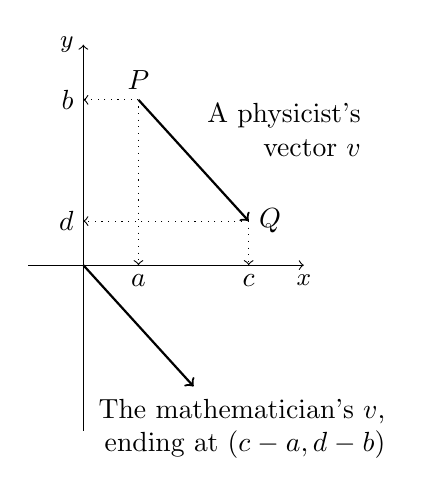
\begin{tikzpicture}[scale=1.4]
\draw[->] (-.5,0) -- (2,0) node[below] {\small $x$};
\draw[->] (0,-1.5) -- (0,2) node[left] {\small $y$};
\draw[->,thick] (1/2,3/2) node[above] {$P$} -- (3/2,2/5) node[right] {$Q$};
\node [text width=2cm,align=right,above right] at (1,18/20) {A physicist's vector $v$};
\draw[dotted,->] (1/2,3/2) -- (1/2,0) node[below] {$a$};
\draw[dotted,->] (1/2,3/2) -- (0,3/2) node[left] {$b$};
\draw[dotted,->] (3/2,2/5) -- (3/2,0) node[below] {$c$};
\draw[dotted,->] (3/2,2/5) -- (0,2/5) node[left] {$d$};
\draw[->,thick] (0,0) -- (1,-11/10);
\node [text width=3.75cm,align=right,below] at (7/5,-9/8) {The mathematician's $v$,\\ ending at $(c-a,d-b)$};
\end{tikzpicture}
\caption{The physicist's vector vs. the mathematician's vector.}
\end{figure}

But it pays to keep in mind that the physicists conception of the vector $V$ with coordinates $c-a$ and $d-b$ could be one of many different arrows, while the mathematician's vector $v$ is the arrow from the point $O = (0,0)$ to the point $(c-a, d-b)$.

Now we have circled back around to a muddle. If a mathematician's vector is always based at $O$, we only need to specify where the head of the vector is\dots which is just a point. So, how is a vector supposed to be different from a point, again?

This confusion of three different, shifting, partially-overlapping interpretations causes some trouble to the new learner.
Professionals tend to pass back and forth between these and use them flexibly to get results.
Once you have gotten used to the ideas, you will, too.
You should watch out for these instances where the words point and vector get interchanged.
If they cause you trouble, remember that we have three different things, which are closely related.

For now, the simplest way to handle things is like this:
\begin{itemize}
\item Ignore the physicist's version of the word vector as much as possible.
\item A point is a location in the plane, and represented by coordinates in the form of an ordered pair of numbers $(a,b)$.
\item A vector is an arrow based at the origin, which can be specified by the coordinates of its head. To keep this separate from the idea of a point, we will write it differently, with the numbers stacked vertically like this: $\smvec{a}{b}$.
\item Always remember that for each point in the plane, there is a unique mathematician's vector which corresponds, and vice versa.
\end{itemize}
With this in mind, we make our first official definition.

\begin{definition} A $2$-vector is a vertical stack of $2$ real numbers, like so:
\[
v = \begin{pmatrix} a \\ b \end{pmatrix}.
\]
The collection of all such $2$-vectors is called \emph{the plane}, and written with this notation: $\R^2$.
\end{definition}

The notation $\R^2$ is often read ``arr-two,'' and many people use that language interchangeably with ``the plane.'' Also, most of the time we will just say ``vector,'' rather than ``$2$-vector.'' 

\section*{Vector Algebra}

Let's return to that glimpse of subtraction we saw in Figure \ref{fig:phys-vec-coords}.
We saw there that for points $P = (a,b)$ and $Q = (c,d)$, the vector $v$ from $P$ to $Q$ has coordinates $c-a$ and $d-b$.
This looks almost like we subtracted the points to get $Q-P = v$.
Can we use that?
The weird part is that it mixes up points and vectors.
So, we will just change viewpoints, and instead think of $P$ and $Q$ as (mathematician's) vectors. To keep things clear, let's introduce new labels.
\[
p = \begin{pmatrix} a \\ b \end{pmatrix}, \quad q = \begin{pmatrix} c \\ d \end{pmatrix}
\]
If we put these together on the plane with the physicist's vector $v$ from $p$ to $q$ and the mathematician's $v$ we see a wonderful triangle, and an extra vector.
\begin{figure}[h]
\centering
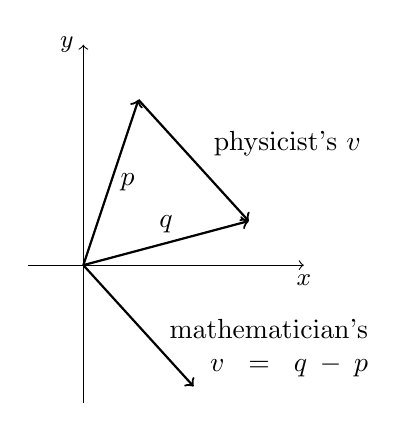
\begin{tikzpicture}[scale=1.4]
\draw[->] (-.5,0) -- (2,0) node[below] {\small $x$};
\draw[->] (0,-1.25) -- (0,2) node[left] {\small $y$};
\draw[->,thick] (1/2,3/2) -- (3/2,2/5);
\node [text width=2cm,align=right,above right] at (1,18/20) {physicist's $v$};
\draw[->,thick] (0,0) -- (1,-11/10);
\node [text width=3.5cm,align=right] at (4/3,-3/4) {mathematician's $v=q-p$};
\draw[->,thick] (0,0) -- (1/2,3/2);
\node[right] at (1/4,3/4) {$p$};
\draw[->,thick] (0,0) -- (3/2,2/5);
\node[above] at (3/4,1/5) {$q$};
\end{tikzpicture}
\caption{Subtraction of vectors}
\label{fig:subtract-vec}
\end{figure}
So we see a way to talk about subtracting vectors: Given two vectors $p$ and $q$ as above, their
\emph{difference} is the vector
\[
V = Q-P = \begin{pmatrix} c \\ d \end{pmatrix} - \begin{pmatrix} a \\ b \end{pmatrix} = \begin{pmatrix} c-a \\ d-b \end{pmatrix}.
\]
Geometrically, we draw the arrow from $p$ to $q$ and then translate it down so that its tail is at the origin $O=(0,0)$. Of course, the order of $p$ and $q$ in this operation matters. If we switch them, we get an arrow pointing in the opposite direction.

If we can subtract vectors, surely we can add vectors. How would that work? Algebraically, if $v=q-p$, then we expect $q=v+p$ by rearranging.
That would mean
\[
q = \begin{pmatrix} c \\ d \end{pmatrix} = v+p = \begin{pmatrix} c-a \\ d-b \end{pmatrix} + \begin{pmatrix} a \\ b \end{pmatrix},
\]
which all fits. It looks like addition should be defined coordinate-by-coordinate.

\begin{definition}[Addition of Vectors]
Let $p = \smvec{a}{b}$ and $q= \smvec{c}{d}$ be two vectors in $\R^2$. Their sum is the vector
\[
p+q = \begin{pmatrix} a+c \\ b+d\end{pmatrix}.
\]
\end{definition}

\begin{theorem}\label{thm:vect-add}
Addition of vectors satisfies the same rules as addition of real numbers:
\begin{compactitem}
\item when adding more than two vectors, it doesn't matter which operations you do first:
$(p+q)+r = p + (q+r)$;
\item one can add in either order $p+q = q+p$;
\item the vector $o$ corresponding to the origin $O$ is a ``zero'' since $p+o = o+p = p$;
\item for each vector $p$, there is an opposite vector $-p$ so that $p + (-p) = o$.
\end{compactitem}
\end{theorem}

Remember that you are supposed to read actively.
You can draw all of these pictures and try out all of these things with specific examples that you invent.
You should check these by making examples and working out the details.
Can you also draw the pictures which go with your examples?

But what about subtracting geometrically? In Figure \ref{fig:subtract-vec}, I have a strong desire to complete the figure by joining the loose end of $v$ to the rest of the figure. If we draw the arrow from the head of $v$ to the head of $q$, we get this:
\begin{figure}[h!]
\centering
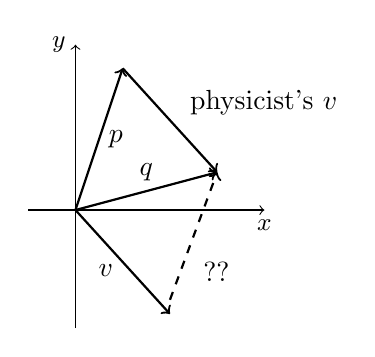
\begin{tikzpicture}[scale=1.2]
\draw[->] (-.5,0) -- (2,0) node[below] {\small $x$};
\draw[->] (0,-1.25) -- (0,1.75) node[left] {\small $y$};
\draw[->,thick] (1/2,3/2) -- (3/2,2/5);
\node [text width=2cm,align=right,above right] at (1,18/20) {physicist's $v$};
\draw[->,thick] (0,0) -- (1,-11/10);
\node [below left] at (1/2,-19/40) {$v$};
\draw[->,thick] (0,0) -- (1/2,3/2);
\node[right] at (1/4,3/4) {$p$};
\draw[->,thick] (0,0) -- (3/2,2/5);
\node[above] at (3/4,1/5) {$q$};
\draw[->,dashed,thick] (1,-19/20) -- (3/2,2/5);
\node[right] at (5/4,-13/20) {??};
\end{tikzpicture}
\caption{Subtraction of vectors}
\label{fig:add-vec}
\end{figure}

What should the label on the dashed vector in Figure \ref{fig:add-vec} be? Just as the physicist's $v$ and the
mathematician's $v$ are parallel, this new vector is parallel to the mathematician's vector $p$.
So the dashed vector must be a physicist's version of $p$. Then we see $q=v+p$.

Now we know how to add geometrically: to add two vectors $u$ and $v$, translate $v$ until its tail is on the head of $u$, then draw a new vector $u+v$ as the vector from the tail of $u$ to the head of this translated $v$. It just repurposes the structure of Figure \ref{fig:add-vec}.

\begin{figure}[h!]
\centering
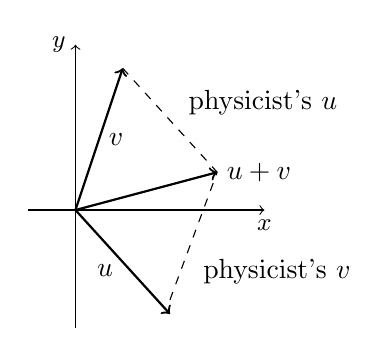
\begin{tikzpicture}[scale=1.2]
\draw[->] (-.5,0) -- (2,0) node[below] {\small $x$};
\draw[->] (0,-1.25) -- (0,1.75) node[left] {\small $y$};
\draw[-,dashed] (1/2,3/2) -- (3/2,2/5);
\node [text width=2cm,align=right,above right] at (1,18/20) {physicist's $u$};
\draw[->,thick] (0,0) -- (1,-11/10);
\node [below left] at (1/2,-19/40) {$u$};
\draw[->,thick] (0,0) -- (1/2,3/2);
\node[right] at (1/4,3/4) {$v$};
\draw[->,thick] (0,0) -- (3/2,2/5);
%\node[above] at (3/4,1/5) {$A+B$};
\draw[-,dashed] (1,-19/20) -- (3/2,2/5) node[right] {$u+v$};
\node[right] at (5/4,-13/20) {physicist's $v$};
\end{tikzpicture}
\caption{Geometric Addition of Vectors}
\label{fig:geom-add-vec}
\end{figure}

This is sometimes called the \emph{parallelogram rule} for addition of vectors.

There is another useful operation on vectors called \emph{scalar multiplication}.
The terminology comes from physics (again) where a \emph{scalar} quantity is just a number, and not a vector.
So ``scalar multiplication'' means to multiply a vector by a scalar.


\begin{definition}[Scalar Multiplication for vectors]
Let $p = \smvec{a}{b}$ be a vector in $\R^2$, and let $\lambda$ be a real number. Then the scalar multiple $\lambda p$ is defined to be
\[
\lambda p = \begin{pmatrix} \lambda a \\ \lambda b \end{pmatrix}
\]
\end{definition}

If you have never seen the symbol $\lambda$ before, it is an old Greek letter pronounced ``lamb-duh.'' It is traditional to use it in linear algebra in lots of places. Welcome to the $\lambda$-club. Oh, there are others, too, like $\mu$, which is pronounced ``myoo.''

Again, this operation has some important similarities to the familiar multiplication of numbers, but because it combines a scalar (a number) with a vector (not a number, exactly) to produce another vector (again, not a number) things are a little different.

\begin{theorem}\label{thm:scalar-mult}
Suppose that $p$ and $q$ are vectors, and $\lambda$ and $\mu$ are numbers. Scalar multiplication has the following properties:
\begin{compactitem}
\item Scalar multiplication distributes over vector addition:\\ $\lambda(p+q) = \lambda p + \lambda q$;
\item Scalar multiplication distributes over scalar addition:\\ $(\lambda + \mu)p = \lambda p + \mu q$;
\item Scalar multiplication and regular multiplication can be done in either order: $\lambda(\mu p) = (\lambda\mu) p$;
\item if $\lambda = 0$, then $\lambda p = 0 p = o$ is the zero vector.
\item if $n$ is a counting number, then $np$ is the same thing as adding together $n$ copies of $p$. In particular, $1p = p$.
\end{compactitem}
\end{theorem}

This Theorem, like the last one, just says that a bunch of natural things you expect to happen really do happen. When you study \textbf{Modern Algebra}, making lists of these kinds of properties will be really useful. So far, we have collected up the properties that describe a \emph{vector space}.


What is the geometry of scalar multiplication?
It corresponds to stretching (or shrinking) a vector, without changing its direction.
Let $\lambda$ be a non-zero number. Since
\[
\lambda p = \lambda \begin{pmatrix} a \\ b \end{pmatrix} = \begin{pmatrix} \lambda a \\ \lambda b\end{pmatrix},
\]
we see that the ratio of the two coordinates of a vector doesn't change under scalar multiplication. This means that $p$ and $\lambda p$ point in the same direction.
One can see this by considering similar triangles with sides parallel to the $x$-axis, the $y$-axis, and $p$.

\begin{figure}[h!]
\centering
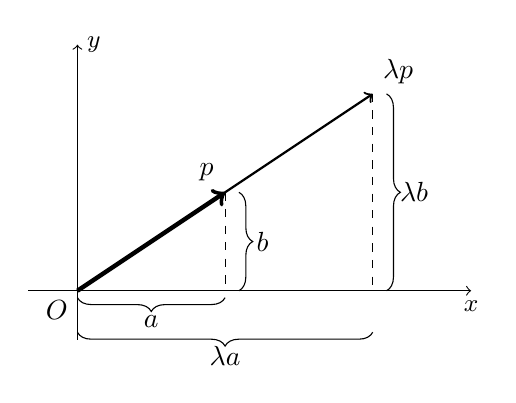
\begin{tikzpicture}[scale=1.25]
\draw[->] (-.5,0) -- (4,0) node[below] {\small $x$};
\draw[->] (0,-.5) -- (0,2.5) node[right] {\small $y$};
\node[below left] at (0,0) {$O$};
\draw[->,thick] (0,0) -- (3,2) node[above right] {$\lambda p$};
\draw[->,ultra thick] (0,0) -- (1.5,1) node[above left] {$p$};
\draw[dashed] (1.5,1) -- (1.5,0);
\draw[dashed] (3,2) -- (3,0);
\draw[decorate,decoration={brace,mirror,amplitude=5pt},xshift=4pt,yshift=0pt] (3,0) -- (3,2) node[midway,xshift=.35cm] {$\lambda b$};
\draw[decorate,decoration={brace,mirror,amplitude=5pt},xshift=4pt,yshift=0pt] (1.5,0) -- (1.5,1) node[midway,xshift=.3cm] {$b$};
\draw[decorate,decoration={brace,mirror,amplitude=5pt},xshift=0pt,yshift=-2pt] (0,0) -- (1.5,0) node[midway,yshift=-.3cm] {$a$};
\draw[decorate,decoration={brace,mirror,amplitude=5pt},xshift=0pt,yshift=-12pt] (0,0) -- (3,0) node[midway,yshift=-.3cm] {$\lambda a$};
\end{tikzpicture}
\caption{Similar triangles and scalar multiplication, $\lambda >1$}
\label{fig:sim-tri}
\end{figure}

The triangles in Figure \ref{fig:sim-tri} are similar: their corresponding horizontal and vertical sides are parallel, and those pairs of sides have a common ratio.
We learn that $p$ and $\lambda p$ lie in the same line.

Now we are getting somewhere! We want to understand lines in the plane, and we have just discovered how scalar multiplication relates to lines which pass through the origin, $O$.

By the way, this picture helps explain the terminology. The vector $\lambda p$ is a rescaled version of $p$. A \emph{scalar} is a thing which \emph{scales} vectors.

\section*{Lines as Parametric Objects}

We see that for a non-zero vector $p$, and a non-zero number $\lambda$, the vectors $p$ and $\lambda p$ lie on the same line through the origin, $O$. But this doesn't depend on which number $\lambda$ we choose. So if we vary $\lambda$, we will get lots of different points on that line.
The picture looks something like this one:
\begin{figure}[h!]
\centering
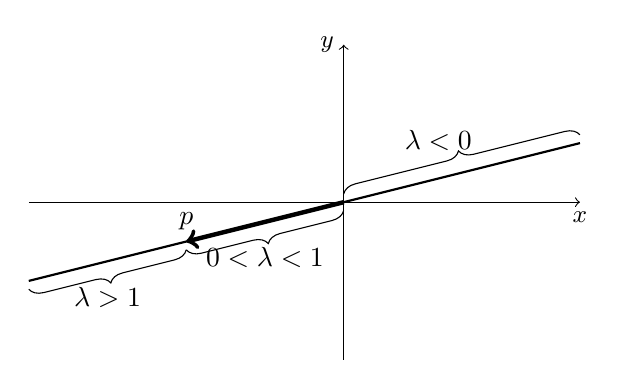
\begin{tikzpicture}
\draw[->] (-4,0) -- (3,0) node[below] {\small $x$};
\draw[->] (0,-2) -- (0,2) node[left] {\small $y$};
\draw[thick] (-4,-1) -- (3,3/4);
\draw[->,ultra thick] (0,0) -- (-2,-1/2) node[above] {$p$};
\draw[decorate,decoration={brace,amplitude=5pt,mirror},xshift=0pt,yshift=-3pt] (-4,-1) -- (-2,-1/2) node[midway,xshift=0cm,yshift=-.35cm] {$\lambda > 1$};
\draw[decorate,decoration={brace,amplitude=5pt,mirror},xshift=0pt,yshift=-3pt] (-2,-1/2) -- (0,0) node[midway,xshift=0cm,yshift=-.35cm] {$0< \lambda <1$};
\draw[decorate,decoration={brace,amplitude=5pt},xshift=0pt,yshift=3pt] (0,0) -- (3,3/4) node[midway,xshift=-.3cm,yshift=.3cm] {$\lambda <0$};
\end{tikzpicture}
\caption{The points on a line: $\lambda p$ for different $\lambda$}
\label{fig:line-scalar}
\end{figure}

This leads us to what is called a \emph{parametric description} of the line.
We think of some variable, say $t$, as a parameter.
(I chose $t$ here so that we think of it as ``time.'')
As we change the value of $t$, the vectors $tp$ trace out the line which goes through the origin and the point which is the head of the vector $p$.

\begin{theorem}[parametric lines through the origin] \label{thm:param-line-origin}
Suppose that $P=(a,b)$ is some point in the plane. The the line which passes through the origin $O$ and the point $P$ consists of the heads of all the vectors
\[
t p = t \begin{pmatrix} a \\ b \end{pmatrix},
\]
where $t$ varies over all real numbers. That is, this line is the set of the heads of all scalar multiples of the vector $p$ corresponding to $P$.
\end{theorem}

This, is fantastic. We can use simple vector algebra to describe any line through the origin.
What about lines that are not through the origin?
Suppose we just have two random points $P$ and $Q$, neither of which is the origin, and we want to describe the line $\ell$ through $P$ and $Q$?

Again, let's think of the points on this line $\ell$ as the heads of mathematics-style vectors.
If we put in the vectors $p$ and $q$ which correspond to the points $P$ and $Q$, we get a good picture like this one.

\begin{figure}[h!]
\centering
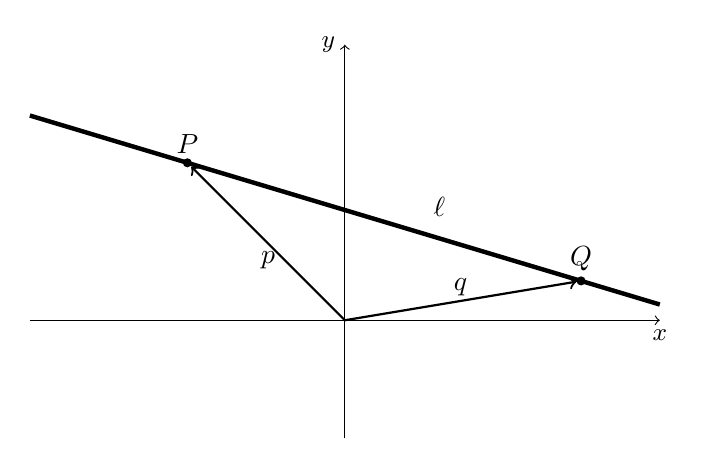
\begin{tikzpicture}[scale=1]
\draw[->] (-4,0) -- (4,0) node[below] {\small $x$};
\draw[->] (0,-1.5) -- (0,3.5) node[left] {\small $y$};
\draw[fill] (-2,2) circle [radius=.05];
\node[above] at (-2,2) {$P$};
\draw[fill] (3,.5) circle [radius=.05];
\node[above] at (3,.5) {$Q$};
\draw[ultra thick] (-4,2.6) -- (4,.2);
\node[above] at (1.2,1.2) {$\ell$};
\draw[->,thick] (0,0) -- (-1.95,1.95) node[midway,yshift=-6pt] {$p$};
\draw[->,thick] (0,0) -- (2.94,.49) node[midway,yshift=5pt] {$q$};
\end{tikzpicture}
\caption{Working toward a parametric line, part 1}
\label{fig:param-line1}
\end{figure}

Each point in Figure \ref{fig:param-line1} is the head of a vector from the origin to that point.
In particular, the point $P$ is the head of the vector $p$.
So if we add $-p$ to every single one of these vectors, we will move the whole line $\ell$ in the direction of $-p$ and with the same distance as $-p$.
That will make a new line, $\ell'$, and the point which comes from $P$ will land on the origin.


\begin{figure}[h!]
\centering
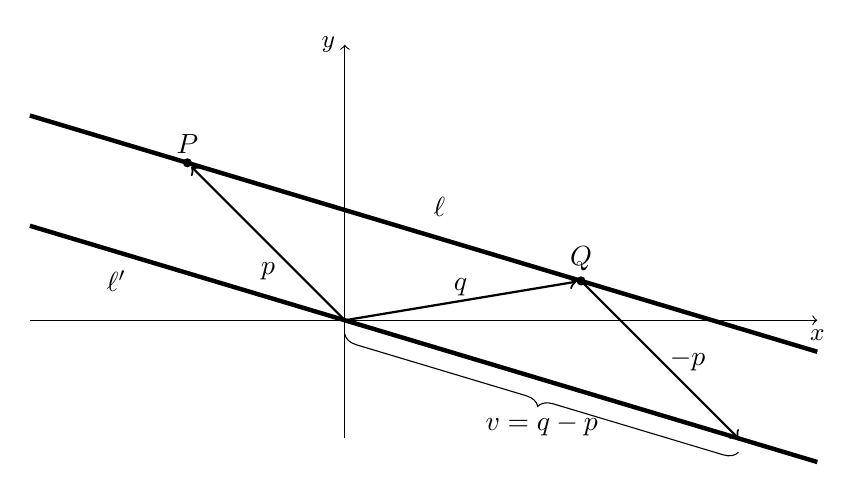
\begin{tikzpicture}[scale=1]
\draw[->] (-4,0) -- (6,0) node[below] {\small $x$};
\draw[->] (0,-1.5) -- (0,3.5) node[left] {\small $y$};
\draw[fill] (-2,2) circle [radius=.05];
\node[above] at (-2,2) {$P$};
\draw[fill] (3,.5) circle [radius=.05];
\node[above] at (3,.5) {$Q$};
\draw[ultra thick] (-4,2.6) -- (6,-.4);
\node[above] at (1.2,1.2) {$\ell$};
\draw[->,thick] (0,0) -- (-1.95,1.95) node[midway,yshift=-10pt] {$p$};
\draw[->,thick] (0,0) -- (2.94,.49) node[midway,yshift=5pt] {$q$};
\draw[ultra thick] (-4,1.2) -- (6,-1.8);
\node at (-2.9,.5) {$\ell'$};
\draw[->,thick] (3,.5) -- (5,-1.5) node[midway,xshift=10pt] {$-p$};
\draw[decorate,decoration={brace,amplitude=5pt,mirror},xshift=0pt,yshift=-5pt] (0,0) -- (5,-1.5) node[midway,yshift=-.41cm] {$v = q-p$};
\end{tikzpicture}
\caption{Working toward a parametric line, part 2}
\label{fig:param-line2}
\end{figure}

Since $q$ is one of the vectors with its head on the original line, the vector $q-p$ will have its head on the new line.
But $q-p$ has its tail at the origin!
So, our new line passes through the origin and the head of the vector $q-p$, and we are in a situation to apply Theorem \ref{thm:param-line-origin}.


By Theorem \ref{thm:param-line-origin}, the line $\ell'$ is described as all of the points which are heads of vectors of the form
$t (q-p)$, where $t$ is a parameter which is allowed to vary over all real numbers.
But we get from $\ell'$ back to $\ell$ by simply adding the vector $p$ back in.
So, our original line $\ell$, which goes through the heads of vectors $p$ and $q$, is described as the set heads of the vectors
\[
p + t (q-p),
\]
where $t$ is a parameter which is allowed to vary over all real numbers.
Now, let's sum up what we have learned.

\begin{theorem}[parametric line]\label{thm:param-line}
Let $P = (a,b)$ and $Q = (c,d)$ be two points in the plane. The line which passes through these two points can be described as the heads of all vectors of the form
\[
p+t(q-p) = \begin{pmatrix} a \\ b \end{pmatrix} + t \begin{pmatrix} c-a \\ d-b\end{pmatrix},
\]
where $t$ is a parameter which is allowed to vary over all real numbers.
\end{theorem}

Note that this theorem actually includes the previous one as a special case.
If one of our points happens to be the origin, we simply use $P=O$, which corresponds to the zero vector, and this description collapses back into the one we found earlier.
In either case, the vector $v= q-p$ is called a \emph{direction vector} for the line.


As a bit of a palate cleanser, let's answer this: Suppose you are given a line described as in the last theorem. How would you sketch it in the plane? The simplest method is to choose two different values of $t$, use them to generate to points on the line, plot those points, and trace the line through them. Which values of $t$ should you choose? It is often convenient to use $t=0$ and $t=1$.

In fact, a parametric description can (perhaps ``should'') be thought of as describing the motion of a vector or point in the plane. 
The parameter $t$ should be thought of as \emph{time}.
As the time changes, the location of the vector (or point) in the plane changes.
This creates a kind of function, which is sometimes written like so:
\[
t \mapsto p + t(q-p)
\]
The input time $t$ is some real number, and the corresponding output is the vector $p+t(q-p)$ in $\R^2$. For any fixed $t$, our function gives us the ``location of the moving point at time $t$.'' You can think of running through all of these different pictures, in sequence, as a movie showing the motion of our vector (or point). Then the line is like a time-lapse photograph which traces out the whole motion.

Note that at time $t=0$, we have the location $0 \mapsto p + 0(q-p) = p$, and at time $t=1$, we get the location $1 \mapsto p+1(q-p) = q$. So it makes sense to think of our parametrized line as describing motion ``from $p$ to $q$.'' And the whole time, the direction of motion is exactly $v=q-p$: from $p$ to $q$ in the physicist's sense.


\section*{Lengths and Angles in the plane}

What should we mean by the ``length'' of a vector $u$ in $\R^2$? The most natural thing is to use the notion of the length of the line segment from the tail to the head --- the regular length of the arrow involved. This natural thing is just what we want, but because we wish to generalize it later, it will be best to give it an unusual name: the \emph{norm} of a vector. 

How shall we understand it? The key comes from looking upon Figure \ref{fig:sim-tri}
with new eyes. There we see a vector in $\R^2$ as the hypotenuse of a right triangle 
having its legs parallel to the two coordinate axes.

\begin{figure}[h!]
\centering
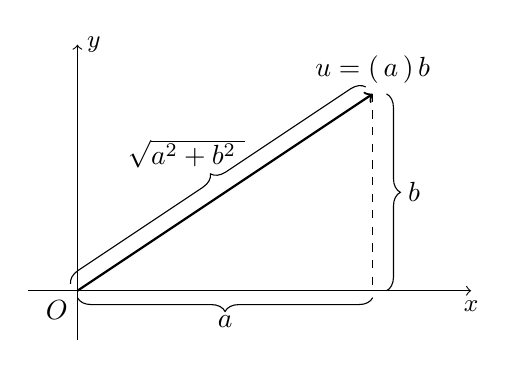
\begin{tikzpicture}[scale=1.25]
\draw[->] (-.5,0) -- (4,0) node[below] {\small $x$};
\draw[->] (0,-.5) -- (0,2.5) node[right] {\small $y$};
\node[below left] at (0,0) {$O$};
\draw[->,thick] (0,0) -- (3,2) node[above] {$u = \begin{pmatrix} a \\ b\end{pmatrix}$};
\draw[dashed] (3,2) -- (3,0);
\draw[decorate,decoration={brace,mirror,amplitude=5pt},xshift=4pt,yshift=0pt] (3,0) -- (3,2) node[midway,xshift=.35cm] {$b$};
\draw[decorate,decoration={brace,mirror,amplitude=5pt},xshift=0pt,yshift=-2pt] (0,0) -- (3,0) node[midway,yshift=-.3cm] {$a$};
\draw[decorate,decoration={brace,amplitude=5pt},xshift=-2pt,yshift=2pt] (0,0) -- (3,2) node[midway,xshift=-.4cm,yshift=.4cm] {$\sqrt{a^2+b^2\ }$};
\end{tikzpicture}
\caption{The Norm of a vector}
\label{fig:norm}
\end{figure}

These two legs then have lengths which are equal to our two coordinates, respectively.
So we can compute the length of the arrow by the Pythagorean Theorem. Now that we understand what we want, we can make our definition.

\begin{definition}[Norm of a vector]
Let $u = \smvec{a}{b}$ be a vector in $\R^2$.
The \emph{norm} of $u$ is the number
\[
\norm{u} = \sqrt{a^2 + b^2\ }.
\]
\end{definition}

It is important to remember that the norm is a number, but never a negative number. Also, the only vector which has norm equal to zero is the zero vector. We shall often have the occasion to use norms of vectors as scalars in forming linear combinations.

As long as we have the concepts of norm and scalar in front of us, let us investigate how those interact. If $\lambda$ is a scalar, then how do the norms a vector $u$ and the rescaled $\lambda u$ compare? Let's write our vector in the form $u=\smvec{a}{b}$. Then we can do the following straightforward computation:
\[
\norm{\lambda u} = \norm{ \lambda \begin{pmatrix} a \\ b \end{pmatrix}} = \norm{ \begin{pmatrix} \lambda a \\ \lambda b \end{pmatrix} } = \sqrt{ (\lambda a)^2 + (\lambda b)^2\ } = |\lambda| \norm{u}
\]
This conforms to our basic ideas about scalar multiplication. If we rescale a vector, we are really just changing its length by that factor. (And then there is the worry over the sign of the scalar, because lengths must not be negative.)


In a terrible linguistic collision, the most useful role for the norm of a vector is in the process of \emph{normalizing} that vector. 
Beware, mathematics has several words that are overused! 
Norm, normal, normalize, normalized and other forms of this are a prime example.
To \emph{normalize} a vector $u$, we multiply it by the scalar $\norm{u}^{-1}$, and thus produce a new vector $u/\norm{u}$ which points in the same direction as $u$, but has norm equal to $1$. This is because we can use our observation just above about how norms interact with scalar multiplication to compute:
\[
\norm{\norm{u}^{-1} u} = \norm{u}^{-1}\norm{u}  = 1.
\]
That last multiplication is just a multiplication of numbers.
Note that all of that only makes sense as long as $u$ is not the zero vector. If $u$ is the zero vector, its norm is $\norm{u}=0$. Since it makes no sense to divide by zero, it is not possible to normalize the zero vector.

Just to make sure all of this stays confusing for learners, mathematicians call a vector with norm equal to $1$ a \emph{unit vector}.

To sum up: given a non-zero vector $u$, it is possible to normalize it, which means to replace it with the vector $u/\norm{u}$, which is a unit vector.


Now that we are talking about proper geometry with length, can we find a way to measure the angle between two vectors? We can, if we use some trigonometry. We will use the following three facts:
\begin{enumerate}
\item Each point on the unit circle can be represented as a point of the form $(\cos(\alpha), \sin(\alpha))$ for some angle $\alpha$ between $0$ and $2\pi$, so the corresponding vector can be written as $p = \smvec{\cos(\alpha)}{\sin(\alpha)}$.


\begin{figure}[h]
\centering
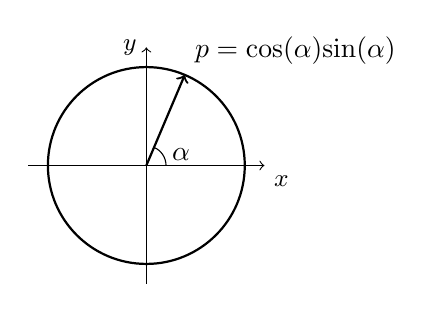
\begin{tikzpicture}[scale=1.25]
\draw[->] (-1.2,0) -- (1.2,0) node[below right] {\small $x$};
\draw[->] (0,-1.2) -- (0,1.2) node[left] {\small $y$};
\draw[thick] (0,0) circle [radius=1];
\draw[thick,->] (0,0) -- (67:1) node[above right] {$p = \smvec{\cos(\alpha)}{\sin(\alpha)}$};
\draw (.2,0) arc [radius=0.2,start angle=0,end angle=67];
\node[right] at (35:.2) {$\alpha$};
\end{tikzpicture}
\caption{Trigonometry for points on the unit circle}
\label{fig:unit-circle}
\end{figure}


\item The function $\theta \mapsto \cos(\theta)$ associates each angle in the interval
$[0,\pi]$ to a unique real number in the interval $[-1,1]$, and vice versa. For us, this means that it to measure an angle, we can get away with instead finding the cosine of that angle.

\begin{figure}[h]
\centering
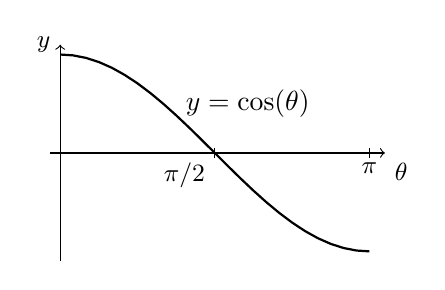
\begin{tikzpicture}[scale=1.25]
\draw[->] (-.1,0) -- (3.3,0) node[below right] {\small $\theta$};
\draw[->] (0,-1.1) -- (0,1.1) node[left] {\small $y$};
\draw [thick,domain=0:pi] plot (\x, {cos(\x r)});
\node[right] at (3*pi/8,1/2) {$y=\cos(\theta)$};
\draw[-] (pi/2,-.05) -- (pi/2,.05);
\draw[-] (pi,-.05) -- (pi,.05);
\node[below left] at (pi/2,0) {\small $\pi/2$};
\node[below] at (pi,0) {\small $\pi$};
\end{tikzpicture}
\caption{Part of the graph of $y=\cos(\theta)$}
\label{fig:cos-graph}
\end{figure}

\item There is an identity on trigonometric functions that helps us deal with the the cosine of a difference of angles: If $\alpha$ and $\beta$ are two angles, then
\[
\cos(\beta-\alpha) = \cos(\alpha)\cos(\beta) + \sin(\alpha)\sin(\beta).
\]
\end{enumerate}

So, let us consider the angle between two vectors, $u$ and $v$, in $\R^2$. 
First, the angle between these vectors does not depend at all on their lengths. 
If we change one, or both, of the vectors by rescaling them, that will not change the directions involved, and hence will not change the angle we seek. 
We can get to a more uniform set up for our task by normalizing $u$ and $v$. 
Thus we will instead consider the unit vectors $u/\norm{u}$ and $v/\norm{v}$, and look for the angle $\theta$ between them.

Since our vectors are unit vectors, we can represent them with trigonometric functions:
\[
\frac{u}{\norm{u}} = \begin{pmatrix} \cos(\alpha)\\ \sin(\alpha) \end{pmatrix}, \qquad
\frac{v}{\norm{v}} = \begin{pmatrix} \cos(\beta)\\ \sin(\beta) \end{pmatrix}.
\]
Let's suppose that the angle $\beta$ that $v$ makes with the $x$-axis is larger than the angle $\alpha$ that $u$ makes with the $x$-axis. Then we want to find the angle $\theta = \beta-\alpha$. 

\begin{figure}[h]
\centering
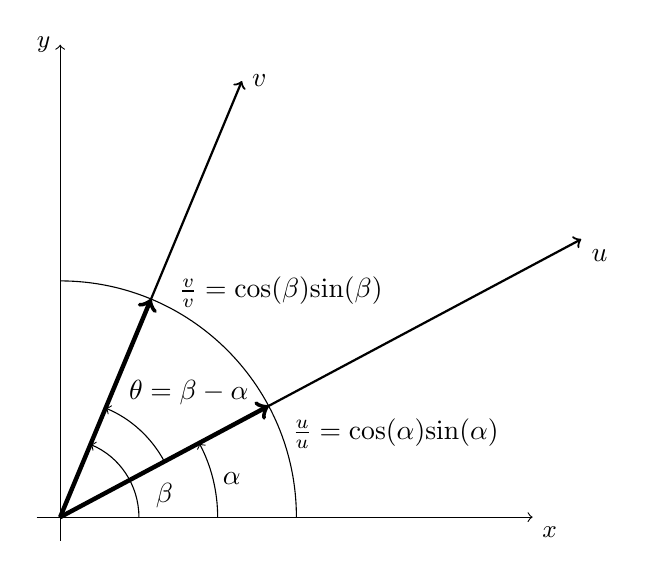
\begin{tikzpicture}[scale=3]
\draw[->] (-.1,0) -- (2,0) node[below right] {\small $x$};
\draw[->] (0,-.1) -- (0,2) node[left] {\small $y$};
\draw (1,0) arc [radius=1,start angle=0,end angle=90];
\draw[thick,->] (0,0) -- (10/13,24/13) node[right] {$v$};
\draw[ultra thick,->] (0,0) -- (5/13,12/13);
\node [above right] at (6/13,11/13) {$\frac{v}{\norm{v}}=\smvec{\cos(\beta)}{\sin(\beta)}$};
\draw[thick,->] (0,0) -- (37.5/17,20/17) node[below right] {$u$};
\draw[ultra thick,->] (0,0) -- (15/17,8/17);
\node [right] at (16/17,6/17) {$\frac{u}{\norm{u}}=\smvec{\cos(\alpha)}{\sin(\alpha)}$};
\draw[->] (2/3,0) arc [radius=2/3,start angle=0,end angle=28];
\node[right] at (14:2/3) {$\alpha$};
\draw[->] (1/3,0) arc [radius=1/3,start angle=0,end angle=67.38];
\node[right] at (14:3/8) {$\beta$};
\draw[->] (28:1/2) arc [radius=1/2,start angle=28,end angle=67.38];
\node[above right] at (60:1/2) {$\theta = \beta - \alpha$};
\end{tikzpicture}
\caption{Finding the angle between two vectors.}
\label{fig:angle-computation}
\end{figure}


Since cosine is such a nice function on $[0,\pi]$, it will do to first try to find $\cos(\theta)$. But then we can simply apply the angle difference formula for cosine to see
\[
\cos(\theta) = \cos(\beta - \alpha) = \cos(\alpha)\cos(\beta) + \sin(\alpha)\sin(\beta).
\]

This is a great situation. To find $\cos(\theta)$, we can just form a funny combination of the components of the vectors $u/\norm{u}$ and $v/\norm{v}$. 


That funny combination takes the form ``product of first components plus product of second components.'' That is familiar! It looks a bit like what happens when we compute a norm, where we have a ``square of the first component plus the square of the second component.'' Motivated by this happy coincidence, we make up a new object to help us organize the similarities:
\begin{definition}[Dot Product]
Let $u = \smvec{u_1}{u_2}$ and $v = \smvec{v_1}{v_2}$ be vectors in $\R^2$. 
The \emph{dot product} of $u$ and $v$ is the number
\[
u\cdot v = u_1v_1 + u_2v_2 .
\]
\end{definition}

The dot product is mysterious for new learners. You take this funny combination of the components, and somehow learn all kinds of information about lengths and angles. The dot product has many useful properties, which we gather together now.

\begin{theorem}\label{thm:dot-prod-props}
Let $u$, $v$, and $w$ be vectors in $\R^2$ and let $\lambda$ and $\mu$ be scalars. Then
\begin{itemize}
\item The angle $\theta$ between $u$ and $v$ is given by 
\[
\theta = \arccos\left(\frac{u\cdot v}{\norm{u}\norm{v}}\right);
\]
\item The norm of $u$ is $\norm{u} = \sqrt{u\cdot u\ }$;
\item The dot product is symmetric: $u\cdot v = v \cdot u$;
\item The dot product distributes over linear combinations 
\[
u \cdot (\lambda v + \mu w) = \lambda (u\cdot v) + \mu (u\cdot w)
\]
\end{itemize}
\end{theorem}

As our study progresses, we will not have much use for measuring particular angles, but it will be very important to us to understand situations when two vectors make an angle of $\pi/2$ radians (i.e. $90^{\circ}$, a right angle). It is common to call such vectors \emph{perpendicular}. It is a fact that $\cos(\pi/2) = 0$, so that non-zero vectors $u$ and $v$ make an angle of $\pi/2$ when
\[
0 = \cos(\pi/2) = \dfrac{u\cdot v}{\norm{u}\norm{v}}.
\]
By clearing out the denominator of this fraction, we see that $u$ and $v$ make an angle of $\pi/2$ exactly when $u\cdot v = 0$.  We will generalize this idea eventually, but it is convenient to start using the proper word now.
\begin{definition}[Orthogonal vectors]
We say that a pair of non-zero vectors $u$ and $v$ are \emph{orthogonal} exactly when $u\cdot v=0$.
\end{definition}
We have to be a little careful and include the caveat that $u$ and $v$ are nonzero, because of course the dot product of any vector with the zero vector is zero (the number, this time), but it does not feel right to say that the zero vector makes an angle of any type with any other vector.

\section*{Normal Vectors and Equations for Lines}

Our discussion of the basic geometry of vectors feels like a digression. It has led us away from our main goal, which is to describe lines in the plane. But now we have enough information to circle back\footnote{This is a geometry joke. I am sorry. But not really.} and use the dot product and the concept of orthogonality to give a different way of describing lines. As before, we will start with the case of lines through the origin.

Suppose that we are given a vector $u = \smvec{a}{b}$. What vectors are orthogonal to $u$? When we try to just sketch this, we get a line through the origin! It looks a lot like Figure \ref{figure:orthogonal-line}.
\begin{figure}[h]
\centering
\begin{tikzpicture}[scale=1.5]
\draw[->] (-2,0) -- (2,0) node[below right] {\small $x$};
\draw[->] (0,-2) -- (0,2) node[left] {\small $y$};
\draw[thick,->] (0,0) -- (1,-2/3) node[right] {$u$};
\draw[thick,domain=-1.25:1.25] plot (\x, {1.5*\x});
\draw (1/5,-2/15) -- (5/15,1/15) node[above right] {Our right angle}-- (2/15,1/5);
\end{tikzpicture}
\caption{The line of vectors orthogonal to $u$.}
\label{figure:orthogonal-line}
\end{figure}


Let's try to be more precise. Suppose we were lucky enough to figure out one single vector $v_0$ which is orthogonal to $u$. Then any scalar multiple $tv_0$ of $v_0$ will also be orthogonal to $u$, because
\[
(tv_0)\cdot u = t(v_0\cdot u) = t(0) = 0.
\]
But the collection of vectors of the form $tv_0$ is the parametric line through the origin. So, the line we seek is the line through the origin with direction $v_0$.

How can we find such a $v_0$? Well, in $\R^2$, we can write $v_0 = \smvec{x}{y}$ and then use the orthogonality condition to see that $x$ and $y$ must satisfy
\[
0 = u\cdot v_0= \begin{pmatrix} a \\ b \end{pmatrix}\cdot \begin{pmatrix} x \\ y \end{pmatrix} = ax +by .
\]
After a little poking around, one can discover that one solution to the equation $ax+by=0$ is $x=-b, y=a$. So we can choose $v_0 = \smvec{-b}{a}$. Of course, there are 
other solutions to this equation (a whole line's worth!), but we just need one and this one is convenient. 

If we collect this sequence of observations, we get the following theorem.

\begin{theorem}[Equation for a line through the origin]
Let $u = \smvec{a}{b}$ be a non-zero vector. Then the set of vectors orthogonal to $u$ is the line with parametric description
\[
t \mapsto t\begin{pmatrix} -b \\ a \end{pmatrix}.
\]

Moreover, we can describe that line by an equation: The line of vectors orthogonal to $u$ consists of the vectors $X = \smvec{x}{y}$ whose coordinates satisfy the equation
\[
ax+by = 0.
\]

On the other hand, for each line $\ell$ through the origin with direction vector $v=\smvec{c}{d}$, the vector $u = \smvec{-d}{c}$ is orthogonal to all of the vectors in the line $\ell$. Furthermore, the line $\ell$ can be represented as the collection of vectors $X=\smvec{x}{y}$ whose coordinates satisfy the equation
\[
-dx + cy=0.
\]
\end{theorem}

\begin{definition}[Normal Vector to a line]
A vector which is orthogonal to all of the direction vectors of a line is called a 
\emph{normal vector} for that line.
\end{definition}

Note that there is a little looseness here in the descriptions. A line has many direction vectors, and also many normal vectors. But there is only so much leeway: all of the direction vectors are scalar multiples of each other, and all of the normal vectors are scalar multiples of each other.


And here we have introduced yet another use for some form of the word ``normal.'' Be aware.


Now that we can write equations to help us describe lines through the origin, we would like to have a similar understanding for lines which do not pass through the origin. First, take any line $\ell$. Then $\ell$ is parallel to a line $\ell'$ which passes through the origin. Using what we know above, pick out a normal vector $u = \smvec{a}{b}$ to the line $\ell'$. Since $\ell$ and $\ell'$ are parallel, $u$ is a normal vector for both. Then, pick out just one vector $p$ which has its head on the line $\ell$. (So the corresponding point $P$ lies on $\ell$.)

If we let some unknown, generic vector with its head on the line $\ell$ be represented by the variable vector $X = \smvec{x}{y}$, we see that the physicist's $X-p$ lies entirely in the line $\ell$. Hence the mathematician's $X-p$ is a direction vector for $\ell$, and therefore orthogonal to the vector $u$. 

\begin{figure}[h]
\centering
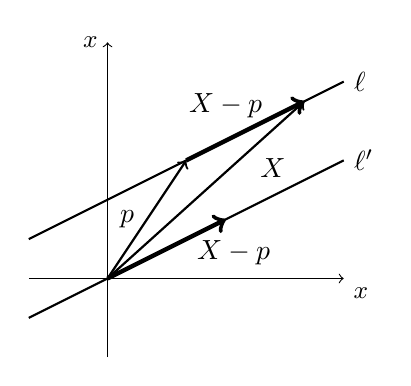
\begin{tikzpicture}[scale=1]
\draw[->] (-1,0) -- (3,0) node[below right] {\small $x$};
\draw[->] (0,-1) -- (0,3) node[left] {\small $x$};
\draw[thick] (-1,-.5) -- (3,3/2) node[right] {$\ell'$};
\draw[thick] (-1,.5) -- (3,5/2) node[right] {$\ell$};
\draw[thick,->] (0,0) -- (1,3/2);
\node at (.25,.75) {$p$};
\draw[thick,->] (0,0) -- (2.5,2.25);
\node at (2.1,1.4) {$X$};
\draw[ultra thick,->] (1,3/2) -- (2.5,2.25);
\node at (1.5,2.2) {$X-p$};
\draw[ultra thick,->] (0,0) -- (1.5,.75);
\node[below] at (1.6,.6) {$X-p$};
\end{tikzpicture}
\caption{Sorting out the equation of a generic line.}
\label{fig:general-line}
\end{figure}


Using the condition for orthogonality, we can derive an equation that the components $x$ and $y$ must satisfy in the following manner. First,
\[
0 = u\cdot (X-p) = u\cdot X - u\cdot p;
\]
therefore,
\[
u\cdot X = u\cdot p.
\]
But $c =u\cdot p$ is just a number. And we have already learned how to re-express $u\cdot X$ as $ax+by$. Rewriting each side of the last displayed equation, we obtain
\[
ax +by = c.
\]

That is the form of an equation for a generic line in the plane. This way of writing the equation of a line in the plane is called the \emph{standard form} of the equation of a line. There are some important features to track in this form:
\begin{itemize}
\item The coefficients $a$ and $b$ of the variables are just the components of the normal vector, but this normal vector is chosen just by looking at a line through the origin. There are a great many lines which are all parallel to the same line through the origin, so they will all have the same set of coefficients.
\item Changing which line in that family of parallel lines will involve changing the point $P$ and the corresponding vector $p$. So even though $a$ and $b$ will not change, the number $c = u\cdot p$ will be different.
\item In each family of parallel lines, the one with right hand side $c=0$ is the one through the origin.
\item Changing the coefficents $a$ and $b$ results in a different normal vector, and hence a different family of parallel lines.
\end{itemize}

\begin{theorem}[Equation of a generic line in the plane]
Suppose that $\ell$ is a line in the plane. Let $P$ be a point on the line, with corresponding vector $p$, and let $u=\smvec{a}{b}$ be a normal vector for $\ell$. Set $c=u\cdot p$.

Then $\ell$ is the collection of points at the heads of the vectors $X = \smvec{x}{y}$ which satisfy the equation
\[
ax+by=c.
\]
\end{theorem}

\section*{Working with Lines Described by Equations}

To make a graph of a line described by an equation, it is easiest to choose two points $P$ and $Q$ which lie on the line, and then draw the line passing through them. In most cases, the most convenient points are the \emph{intercepts} where the line meets the coordinate axes. If the line is $ax+by=c$, then we can find the $x$-intercept by setting $y=0$ and solving for $x=c/a$. Hence the point of interest is $P=(c/a,0)$. Similarly, the $y$-intercept can be found by setting $x=0$. The resulting point will be $Q=(0,c/b)$.
Then it is no trouble to plot these two points and draw a line through them.

Now, suppose we have a line described parametrically. We can find the equation of that line by a process known as ``eliminating the parameter.'' If the parametric form is
\[
t \mapsto \begin{pmatrix} p_0 \\ p_1 \end{pmatrix} + t \begin{pmatrix} v_0 \\ v_1 \end{pmatrix}, 
\]
we take apart the two coordinates of the vector to form a pair of parametric equations
\[
\left\{\begin{array}{rrrrr} x & = & p_0 & + & tv_0 \\ y & = & p_1 & + & tv_1 \end{array}\right.
\]
Now, we multiply through the first equation by $-v_1$ and the second equation by $v_0$
\[
\left\{\begin{array}{rrrrr} -v_1 x & = & -v_1 p_0 & - & tv_0 v_1 \\ v_0 y & = & v_0  p_1 & + & tv_0 v_1 \end{array}\right. ,
\]
and then we add the two equations, thus eliminating the appearance of the parameter $t$, to obtain
\[
-v_1 x + v_0 y = -v_1p_0 + v_0p_1.
\]
This is the equation of the line.

Finally, suppose we have an equation of the line, and we wish to find a parametric representation for it. There is a simple process for doing so, with a neat little trick in the heart of it.

Let our equation be $ax+by=c$, and assume for simplicity that $a\neq 0$. Then, with a little bit of manipulation, we may rewrite the equation as 
\[
x = \frac{c}{a} - y \frac{b}{a}.
\]
The trick is to treat the variable $y$ as if it was our parameter. That is, just declare $y=t$. That gives us a pair of equations, which we can write as
\[
\left\{ \begin{array}{rrrrl} x & = & \frac{c}{a} & - & t\frac{b}{a} \\ y & = & & & t\end{array}\right. .
\]
Now, written this way, it is not too hard to translate this into a vector parametric form for the line.
\[
\begin{pmatrix} x \\ y \end{pmatrix} = \begin{pmatrix} c/a \\ 0 \end{pmatrix} + t \begin{pmatrix} -b/a \\ 1 \end{pmatrix},
\]
or
\[
t \mapsto \begin{pmatrix} c/a \\ 0 \end{pmatrix} + t \begin{pmatrix} -b/a \\ 1 \end{pmatrix} .
\]
If you like, you can rescale that direction vector, and instead write
\[
t \mapsto \begin{pmatrix} c/a \\ 0 \end{pmatrix} + t \begin{pmatrix} -b \\ a \end{pmatrix} .
\]
Later it will be important to us that the direction vector $\smvec{-b}{a}$ is a solution to the associated equation $ax+by=0$.



\end{document}
